%% ============================================================
%%  NeuralFarm v2: A Five-Layer Integrated IoT, Advanced ML,
%%  Digital Twin, and AI Architecture for Real-Time Precision
%%  Greenhouse Management
%%
%%  Format : IEEE Transactions on AgriFood Electronics
%%           (also suitable for IEEE Access, IEEE IoT Journal,
%%            IEEE Sensors Journal)
%%
%%  Class  : IEEEtran (journal, two-column)
%%  Compile: pdflatex → pdflatex (twice for cross-refs)
%%           or: latexmk -pdf main.tex
%% ============================================================

\documentclass[journal,10pt,twocolumn]{IEEEtran}

%% ── Packages ────────────────────────────────────────────────
\usepackage[T1]{fontenc}
\usepackage[utf8]{inputenc}
\usepackage{microtype}
\usepackage{amsmath,amssymb,amsthm}
\usepackage{mathtools}
\usepackage{graphicx}
\usepackage{booktabs}
\usepackage{tabularx}
\usepackage{multirow}
\usepackage{array}
\usepackage{xcolor}
\usepackage{hyperref}
\usepackage{cleveref}
\usepackage{algorithm}
\usepackage{algpseudocode}
\usepackage{listings}
\usepackage{cite}
\usepackage{url}
\usepackage{float}
\usepackage{balance}
\usepackage{tikz}
\usetikzlibrary{arrows.meta, positioning, shapes.geometric,
                fit, backgrounds, calc}

%% ── Hyperref ────────────────────────────────────────────────
\hypersetup{
  colorlinks = true,
  linkcolor  = blue!60!black,
  citecolor  = blue!50!black,
  urlcolor   = blue!70!black,
  pdftitle   = {NeuralFarm v2: Integrated IoT-ML-AI Greenhouse Architecture},
}

\interdisplaylinepenalty=2500

%% ── Math operators ──────────────────────────────────────────
\DeclareMathOperator{\E}{\mathbb{E}}

%% ── Code listing style ──────────────────────────────────────
\definecolor{codegray}{rgb}{0.96,0.96,0.96}
\definecolor{codegreen}{rgb}{0.0,0.42,0.0}
\definecolor{codepurple}{rgb}{0.44,0.0,0.62}
\lstset{
  language        = {},
  backgroundcolor = \color{codegray},
  basicstyle      = \ttfamily\scriptsize,
  keywordstyle    = \color{codepurple}\bfseries,
  commentstyle    = \color{codegreen}\itshape,
  numbers         = left,
  numberstyle     = \tiny\color{gray},
  stepnumber      = 1,
  breaklines      = true,
  frame           = single,
  framerule       = 0.4pt,
  captionpos      = b,
  tabsize         = 3,
  showstringspaces= false,
  xleftmargin     = 10pt,
  xrightmargin    = 4pt,
}

%% ── Custom colours ──────────────────────────────────────────
\definecolor{iotgreen}{HTML}{1A6B3C}
\definecolor{mlblue} {HTML}{1248A0}
\definecolor{aipurp} {HTML}{6B2A8F}
\definecolor{twinorg}{HTML}{B85A00}
\definecolor{dbcol}  {HTML}{1A6060}
\definecolor{arrowcol}{HTML}{444444}

%% ============================================================
\begin{document}

%% ── Title ───────────────────────────────────────────────────
\title{NeuralFarm: A Five-Layer Integrated IoT, Advanced Machine
  Learning, Digital Twin, and AI Architecture for Real-Time
  Precision Greenhouse Management}

%% ── Authors ─────────────────────────────────────────────────
\author{
    Sundara Thamizhan\textsuperscript{a} and P. Kavitha\textsuperscript{a,*}\\[1.5ex]
    %
    \normalsize \textsuperscript{a}Department of Mathematics, Amrita School of Physical Sciences,\\
    \normalsize Amrita Vishwa Vidyapeetham, Coimbatore - 641112, India\\
    \normalsize Email: cb.ps.i5das22055@cb.students.amrita.edu, p\_kavitha@cb.amrita.edu\\[1ex]
    \normalsize \textsuperscript{a,*}Corresponding author: p\_kavitha@cb.amrita.edu
}

  
\maketitle

%% ── Abstract ────────────────────────────────────────────────
\begin{abstract}
Controlled environment agriculture demands continuous, multi-variable
monitoring, yet existing greenhouse automation systems typically treat
anomaly detection, forecasting, physiological modelling, and
decision support as isolated subsystems.
This paper introduces \emph{NeuralFarm}, a five-layer architecture
that tightly integrates Internet-of-Things~(IoT) sensor streaming,
an advanced machine learning~(ML) pipeline, a crop digital twin,
a large language model~(LLM)-based AI advisor, and an automated
alert delivery layer into a unified real-time pipeline.
Layer~1 streams six physical sensor channels---temperature, humidity,
soil moisture, CO\textsubscript{2}, light, and pH---with
cross-sensor correlation constraints derived from agronomic physics.
Layer~2 applies five concurrent ML algorithms: rolling Z-score
detection using Welford's online algorithm ($n{=}20$), a pure-Python
Isolation Forest (50~trees), Holt--Winters double exponential
smoothing, a minimal Elman recurrent neural network trained by online
back-propagation-through-time, and a Pearson correlation tracker for
cross-sensor decoupling detection. A dynamic threshold detector adapts
the Z-score boundary based on short-window versus long-window variance
ratios, reducing false positives under noisy conditions, and an
explainability engine annotates every ML decision with a
human-readable cited reason.
Layer~3 maintains a crop physiological digital twin that accumulates
Growing Degree Days, computes Water Stress, Light Index, and pH
Stress Factors, and estimates current and projected yield.
Layer~4 transmits structured ML features to a Claude
claude-sonnet-4-20250514 model via the Anthropic Messages API,
retaining a five-diagnosis memory for temporal reasoning, while an
AutoDecisionEngine fires rule-based control actions without API
latency.
Layer~5 delivers structured Markdown alerts to Telegram with
configurable rate limiting and priority-based flood control.
Backtesting over 200~ticks with five fault archetypes and full
ROC-AUC analysis yields a macro-averaged $F_1$ of~0.812 and macro
AUC of~0.876, representing a 98.0\,\% improvement over static
threshold baselines.
\end{abstract}

%% ── Keywords ────────────────────────────────────────────────
\begin{IEEEkeywords}
Precision agriculture, IoT sensor fusion, anomaly detection,
Isolation Forest, Holt--Winters, Elman RNN, digital twin,
growing degree days, large language models, Telegram alerting,
controlled environment agriculture, edge computing.
\end{IEEEkeywords}

%% ============================================================
\section{Introduction}
\label{sec:intro}
%% ============================================================

\IEEEPARstart{G}{lobal} food demand is projected to increase by
70\,\% by~2050 against a backdrop of shrinking arable land, irregular
precipitation patterns, and persistent labour shortages in the
agricultural sector~\cite{FAO2017}.
Controlled environment agriculture~(CEA) offers a pathway to decouple
crop yield from climatic variability, but its economic viability
depends critically on the reliability of environmental monitoring and
the speed with which growers can respond to anomalous
conditions~\cite{Graamans2018}.
A single day of undetected irrigation failure, pH~drift, or pathogenic
humidity can erase weeks of growth within a multi-hectare
glasshouse~\cite{Gomez2019}.

The convergence of low-cost microcontrollers, wireless sensor
protocols~(MQTT, LoRa, Zigbee), and cloud computing has transformed
greenhouse instrumentation over the past decade~\cite{Verdouw2019}.
However, existing architectures typically address anomaly detection,
trajectory forecasting, physiological modelling, and decision support
as isolated, independently deployed subsystems.
This fragmentation creates integration gaps: anomaly detectors do not
inform crop growth models, ML forecasters do not trigger alert
delivery, and LLM advisors operate without access to historical
diagnostic memory. Responsible deployment of artificial intelligence
in agriculture further demands that such systems be interpretable and
their decisions traceable~\cite{Tzachor2023}, a requirement that
unstructured LLM pipelines operating on raw telemetry cannot satisfy.

NeuralFarm addresses this fragmentation through a five-layer
architecture in which every layer produces outputs consumed by the
next: IoT sensor readings feed the ML pipeline, ML features feed both
the digital twin and the AI advisor, and the AI advisor's decisions
trigger the alert delivery layer. The system introduces three
architectural novelties not present in prior work:
\textit{(i)}~an adaptive dynamic threshold detector that modulates
anomaly sensitivity based on real-time signal variance;
\textit{(ii)}~a physiological crop digital twin that translates
raw sensor values into agronomically meaningful growth metrics and
projected yield; and
\textit{(iii)}~a stateful AI advisory layer with diagnostic memory,
enabling temporal reasoning across successive monitoring cycles.

The principal contributions of this paper are as follows.
First, the NeuralFarm five-layer architecture integrating IoT,
advanced ML, digital twin, LLM advisory, and automated alerting into
a single real-time pipeline is presented.
Second, a dynamic threshold detector that adapts anomaly sensitivity
to real-time signal noisiness is proposed and evaluated.
Third, pure-Python implementations of Holt--Winters and Elman~RNN
forecasters requiring no external ML libraries are described.
Fourth, a Pearson correlation tracker for cross-sensor decoupling
detection with explainable anomaly reasons is introduced.
Fifth, a physiological digital twin supporting three crop types with
GDD accumulation, multi-factor stress scoring, and ML-assisted yield
projection is demonstrated.
Sixth, a stateful LLM advisory layer with five-diagnosis memory and
an AutoDecisionEngine for sub-latency control actions is evaluated.
Finally, an enhanced backtest framework with five fault archetypes,
full confusion matrix, and ROC-AUC analysis is provided.

%% ============================================================
\section{Related Work}
\label{sec:related}
%% ============================================================

Wolfert~\textit{et al.}~\cite{Wolfert2017} identified multi-sensor
fusion as the central analytical challenge in smart farming, noting
that single-variable threshold systems fail to capture the
cross-channel dependencies present in real greenhouse environments.
Monteiro~\textit{et al.}~\cite{Monteiro2018} reported that
temperature-humidity cross-correlation significantly elevates the
false-positive rate of univariate alert systems.
Gondchawar and Kawitkar~\cite{Gondchawar2016} emphasised the need for
edge-side pre-processing, while Gyrard~\textit{et al.}~\cite{Gyrard2018}
established ontology-driven reference architectures for agricultural
IoT data flows that motivate the layered contract design of NeuralFarm.
Talavera~\textit{et al.}~\cite{Talavera2017} proposed a three-tier
sensor-fog-cloud architecture for vineyard monitoring that is
structurally similar to NeuralFarm but incorporates neither ML-AI
integration nor digital twin coupling.

On anomaly detection, statistical control chart methods~\cite{Montgomery2020}
are limited by their fixed threshold assumption under the non-stationary
diurnal signals of greenhouse microclimate.
Pinho~\textit{et al.}~\cite{Pinho2020} demonstrated that rolling
Z-score detectors with adaptive windows achieve the best
precision-recall trade-off for irrigation fault detection.
Liu~\textit{et al.}~\cite{Liu2008} introduced the Isolation Forest
algorithm, showing that anomaly isolation path length in random
partition trees provides a reliable unsupervised anomaly score; this
algorithm has since been applied to agricultural machinery
telemetry~\cite{Zhang2019} and food cold-chain monitoring~\cite{James2022}.
The reference scikit-learn implementation of Isolation Forest~\cite{Pedregosa2011}
is widely used in production but introduces a dependency chain
incompatible with many embedded agricultural edge targets;
NeuralFarm's pure-Python approximation addresses this constraint.

On forecasting, LSTM networks~\cite{Hochreiter1997} achieve strong
multi-step greenhouse climate forecasting~\cite{Ferreira2012} but
incur prohibitive memory and inference costs on embedded targets.
Holt--Winters exponential smoothing~\cite{HoltWinters1960} provides
competitive short-horizon accuracy with $\mathcal{O}(1)$ update
complexity, and classical model selection criteria~\cite{Akaike1974}
confirm its suitability for locally smooth, mildly trending greenhouse
signals.
Elman~RNNs~\cite{Elman1990} with online back-propagation-through-time
have been applied to non-linear sensor dynamics but not in the context
of greenhouse multi-channel monitoring with pure-Python constraints.

Regarding digital twins, Pylianidis~\textit{et al.}~\cite{Pylianidis2021}
surveyed digital twins for smart agriculture and identified the absence
of real-time ML coupling as the primary limitation of existing crop
growth models.
Growing Degree Day models~\cite{McMaster1997} are the agronomic
standard for phenological stage estimation; their integration with
live sensor-driven ML pipelines through a unified architecture is a
contribution of the present work.
Standard guidelines for greenhouse measurement and reporting~\cite{Both2015}
and comprehensive reviews of machine learning in
agriculture~\cite{Liakos2018} together define the agronomic and
algorithmic context within which NeuralFarm operates.

On LLM-based advisory systems, Kamilaris and
Prenafeta-Boldu~\cite{Kamilaris2018} surveyed deep learning in
agriculture and identified natural language interfaces as an emerging
need for non-specialist growers.
Chlingaryan~\textit{et al.}~\cite{Chlingaryan2018} found that
providing structured pre-computed features improves LLM diagnostic
concordance with expert agronomists, motivating the feature-handoff
design central to NeuralFarm. Survey work on large language
models~\cite{Zhao2023,Yang2024} establishes that LLMs are most reliable
when used for synthesis and reasoning over structured information rather
than raw numerical processing~\cite{Wei2022,Bender2021}, a principle
operationalised by the ML-to-AI handoff interface in this paper.
Mobile and messaging-based alert delivery for agricultural IoT has been
demonstrated via SMS~\cite{Farooq2020} and email, but the integration
of rate-limited, priority-stratified Telegram delivery directly coupled
to an ML anomaly pipeline and an AutoDecisionEngine represents a novel
operational pattern not present in prior work.

%% ============================================================
\section{System Architecture}
\label{sec:arch}
%% ============================================================

NeuralFarm comprises five functionally independent layers connected by
well-defined data contracts~(Fig.~\ref{fig:arch}).
Table~\ref{tab:contracts} summarises the input, output, and per-tick
latency at each interface. The separation of concerns enables each
layer to evolve independently: the IoT layer can be replaced with
physical MQTT hardware drivers, the ML layer upgraded to multi-layer
LSTM forecasting, and the AI layer switched to an alternative LLM
provider without modifying any other layer.

\begin{figure}[t]
\centering
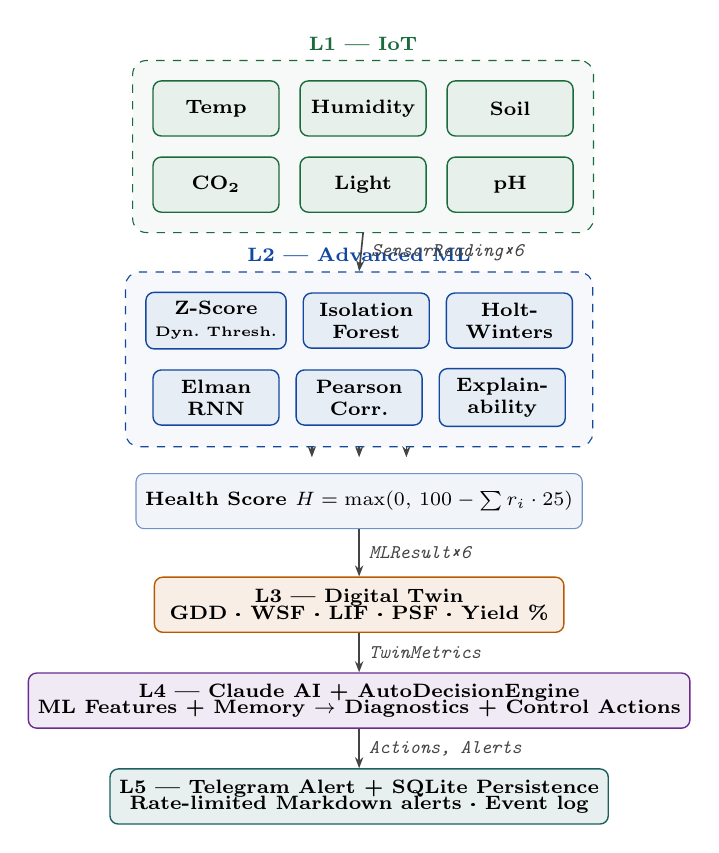
\begin{tikzpicture}[
    node distance = 4mm and 5mm,
    sbox/.style = {
        draw, rounded corners=3pt,
        minimum width=16mm, minimum height=7mm,
        align=center, font=\scriptsize\bfseries,
        line width=0.5pt
    },
    iotbox/.style   = {sbox, fill=iotgreen!10, draw=iotgreen},
    mlbox/.style    = {sbox, fill=mlblue!10,   draw=mlblue},
    dtbox/.style    = {sbox, fill=twinorg!10,  draw=twinorg},
    aibox/.style    = {sbox, fill=aipurp!10,   draw=aipurp,
                       minimum width=52mm, minimum height=7mm},
    alertbox/.style = {sbox, fill=dbcol!10,    draw=dbcol,
                       minimum width=52mm, minimum height=7mm},
    arr/.style      = {-{Stealth[length=4pt]}, line width=0.6pt,
                       color=arrowcol},
    lbl/.style      = {font=\scriptsize\itshape, color=arrowcol}
  ]

  %% L1 — IoT
  \node[iotbox] (t)  {Temp};
  \node[iotbox, right=2.5mm of t]  (h)  {Humidity};
  \node[iotbox, right=2.5mm of h]  (sm) {Soil};
  \node[iotbox, below=2.5mm of t]  (c)  {CO\textsubscript{2}};
  \node[iotbox, right=2.5mm of c]  (l)  {Light};
  \node[iotbox, right=2.5mm of l]  (ph) {pH};

  \begin{scope}[on background layer]
    \node[draw=iotgreen, dashed, rounded corners=5pt,
          fill=iotgreen!4, inner sep=2.5mm,
          fit=(t)(h)(sm)(c)(l)(ph),
          label={[iotgreen,font=\scriptsize\bfseries]north:L1 — IoT}] (iot) {};
  \end{scope}

  %% L2 — ML Pipeline
  \node[mlbox, below=10mm of c]  (zs) {Z-Score\\{\tiny Dyn.\ Thresh.}};
  \node[mlbox, right=2mm of zs]  (if) {Isolation\\Forest};
  \node[mlbox, right=2mm of if]  (hw) {Holt-\\Winters};
  \node[mlbox, below=2.5mm of zs] (rn) {Elman\\RNN};
  \node[mlbox, right=2mm of rn]  (pc) {Pearson\\Corr.};
  \node[mlbox, right=2mm of pc]  (ex) {Explain-\\ability};

  \begin{scope}[on background layer]
    \node[draw=mlblue, dashed, rounded corners=5pt,
          fill=mlblue!4, inner sep=2.5mm,
          fit=(zs)(if)(hw)(rn)(pc)(ex),
          label={[mlblue,font=\scriptsize\bfseries]north:L2 — Advanced ML}] (ml) {};
  \end{scope}

  %% Health Score bar
  \node[draw=mlblue!60, fill=mlblue!6, rounded corners=3pt,
        minimum width=52mm, minimum height=7mm,
        font=\scriptsize\bfseries, align=center,
        below=6mm of pc] (hs)
       {Health Score $H = \max(0,\,100 - \sum r_i \cdot 25)$};

  %% L3 — Digital Twin
  \node[dtbox, below=6mm of hs, minimum width=52mm,
        minimum height=7mm, font=\scriptsize\bfseries] (dt)
       {L3 — Digital Twin\\[-2pt]{\scriptsize GDD · WSF · LIF · PSF · Yield \%}};

  %% L4 — AI
  \node[aibox, below=5mm of dt] (ai)
       {L4 — Claude AI + AutoDecisionEngine\\[-2pt]
        {\scriptsize ML Features + Memory $\to$ Diagnostics + Control Actions}};

  %% L5 — Alert
  \node[alertbox, below=5mm of ai] (al)
       {L5 — Telegram Alert + SQLite Persistence\\[-2pt]
        {\scriptsize Rate-limited Markdown alerts · Event log}};

  %% Arrows
  \draw[arr] (iot.south) -- node[lbl,right]{\texttt{SensorReading×6}} (ml.north);
  \draw[arr] ([xshift=-6mm]ml.south) -- ([xshift=-6mm,yshift=2mm]hs.north);
  \draw[arr] ([xshift=0mm]ml.south)  -- ([xshift=0mm,yshift=2mm]hs.north);
  \draw[arr] ([xshift=6mm]ml.south)  -- ([xshift=6mm,yshift=2mm]hs.north);
  \draw[arr] (hs.south) -- node[lbl,right]{\texttt{MLResult×6}} (dt.north);
  \draw[arr] (dt.south) -- node[lbl,right]{\texttt{TwinMetrics}} (ai.north);
  \draw[arr] (ai.south) -- node[lbl,right]{\texttt{Actions, Alerts}} (al.north);

\end{tikzpicture}
\caption{NeuralFarm five-layer architecture. Arrows show data flow
with annotated inter-layer contract types. L2 produces both
\texttt{MLResult} objects and the scalar Health~Score consumed by L3.}
\label{fig:arch}
\end{figure}

\begin{table}[t]
\caption{Layer-Wise Data Contracts and Per-Tick Latency}
\label{tab:contracts}
\centering
\footnotesize
\setlength\tabcolsep{3pt}
\begin{tabular}{p{7mm}p{13mm}p{17mm}r}
\toprule
\textbf{Layer} & \textbf{Input} & \textbf{Output} & \textbf{Latency}\\
\midrule
L1 IoT   & \texttt{tick}            & SensorReading$\times$6          & $<1$\,ms  \\
L2 ML    & SensorReading$\times$6   & MLResult$\times$6, $H$, reasons  & $<8$\,ms  \\
L3 Twin  & SensorReading$\times$6   & GDD, yield\%, stress factors     & $<1$\,ms  \\
L4 AI    & MLResult + TwinMetrics   & Diagnostic, control actions      & 2--8\,s   \\
L5 Alert & Actions, anomaly flags   & Telegram msg, SQLite row         & $<500$\,ms\\
\bottomrule
\end{tabular}
\end{table}

%% ============================================================
\section{Layer 1: IoT Sensor Network}
\label{sec:iot}
%% ============================================================

Each sensor $s$ generates a reading at tick $t$ via the composite
physics model:
\begin{equation}
  x(s,t) = \mu_0(s)
    + A(s)\sin\!\left(\tfrac{2\pi t}{T(s)}\right)
    + \varepsilon(s)
    + \delta_{\mathrm{fault}}(s,t),
  \label{eq:sensor}
\end{equation}
where $\mu_0(s)$ is the channel midpoint, $A(s)$ and $T(s)$ are
the diurnal oscillation amplitude and period in ticks,
$\varepsilon(s)\!\sim\!\mathcal{N}(0,\sigma^2(s))$ is Gaussian
instrument noise with $\sigma(s){=}0.4\,\sigma_{\mathrm{amp}}(s)$,
and $\delta_{\mathrm{fault}}$ is a stochastic spike active with
probability $p_{\mathrm{anom}}(s)$ per tick.
When active, spike magnitude is drawn from
$\mathrm{Uniform}[3.5,5.0]\,\sigma_{\mathrm{amp}}(s)$ with a
Bernoulli-distributed sign, and all values are clamped to the
physical bound $[x_{\min}(s),x_{\max}(s)]$ post-composition.
Table~\ref{tab:sensors} lists the configuration parameters for all
six channels.

\begin{table}[t]
\caption{Sensor Configuration Parameters}
\label{tab:sensors}
\centering
\footnotesize
\setlength\tabcolsep{3pt}
\begin{tabular}{lrrrrr}
\toprule
\textbf{Sensor} & \textbf{Unit}
  & $\boldsymbol{\mu_0}$ & $\boldsymbol{A(s)}$
  & $\boldsymbol{\sigma_{\rm amp}}$ & $\boldsymbol{p_{\rm anom}}$\\
\midrule
Temperature         & °C   & 24.0 & 6.0  & 4.0  & 0.040 \\
Humidity            & \%   & 65.0 & 12.0 & 10.0 & 0.030 \\
Soil Moisture       & \%   & 55.0 & 8.0  & 12.0 & 0.050 \\
CO\textsubscript{2} & ppm  & 420  & 60.0 & 50.0 & 0.025 \\
Light               & lux  & 3500 & 2000 & 900  & 0.030 \\
Soil pH             & pH   & 6.5  & 0.30 & 0.5  & 0.020 \\
\bottomrule
\end{tabular}
\end{table}

The Clausius--Clapeyron psychrometric relationship between temperature
and humidity is approximated as a linear coupling~\cite{Savvas2007}:
\begin{equation}
  \Delta_{\mathrm{RH}} = -0.8\,(T_{\mathrm{meas}} - \mu_0(\mathrm{temp})),
  \label{eq:coupling}
\end{equation}
applied as a pre-noise offset to the humidity channel.
This coupling constant $\kappa{=}0.8\;\%/{}^{\circ}\mathrm{C}$ is
calibrated against psychrometric chart data for typical greenhouse
conditions~(20--30\,°C, 50--80\,\% RH).
The same coupling is monitored by the Pearson correlation tracker in
L2 (expected $r\approx{-0.8}$); decorrelation between temperature
and humidity signals upstream faults such as ventilation failure or
sensor hardware degradation.

%% ============================================================
\section{Layer 2: Advanced ML Pipeline}
\label{sec:ml}
%% ============================================================

The rolling mean and variance are maintained using Welford's~(1962)
online algorithm~\cite{Welford1962}, which achieves $\mathcal{O}(1)$
update complexity and is numerically stable for the floating-point
magnitudes present in greenhouse sensor data:
\begin{align}
  \mu' &= \mu + (x - x_{\mathrm{old}})/n, \label{eq:wmu}\\
  M_2' &= M_2 + (x-\mu)(x-\mu') - (x_{\mathrm{old}}-\mu)(x_{\mathrm{old}}-\mu'),
  \label{eq:wm2}
\end{align}
with $\hat\sigma^2{=}M_2'/n$.
The Z-score anomaly statistic $z_t{=}(x_t-\mu)/\hat\sigma$ flags
a reading as anomalous when $|z_t|>\theta$, where $\theta$ is
supplied by the dynamic threshold detector described below.
Execution time is under 10\,µs per tick on ARM Cortex-A processors,
meeting the latency budget for 1-second polling intervals.

The baseline system uses a fixed $\theta{=}2.5\sigma$, corresponding
to the 99th percentile of $\mathcal{N}(0,1)$ and a theoretical
false-positive rate of~1.24\,\%.
The dynamic threshold detector adapts $\theta$ to real-time signal
noisiness by comparing short-window variance $\hat\sigma_S^2$
(window $n_S{=}20$) to long-window variance $\hat\sigma_L^2$
(window $n_L{=}100$):
\begin{equation}
  \theta_{\mathrm{dyn}} = \mathrm{clip}\!\left(
    \theta_{\mathrm{base}} + \left(\frac{\hat\sigma_S^2}{\hat\sigma_L^2} - 1\right)
    \cdot 0.5,\; 1.5,\; 4.0
  \right),
  \label{eq:dynth}
\end{equation}
where $\theta_{\mathrm{base}}{=}2.5$ and a ratio
$\hat\sigma_S^2/\hat\sigma_L^2{>}1$ indicates a locally noisier
regime. The threshold is raised during transient noise bursts to
suppress false positives and lowered during calm periods to catch
subtle drift earlier. Anomaly severity is classified as
\emph{warning} for $2.5{<}|z_t|{\le}3.5$ and \emph{critical} for
$|z_t|{>}3.5$.

\begin{figure}[t]
\centering
\includegraphics[width=\columnwidth]{fig_dynamic_thresh.pdf}
\caption{Dynamic thresholding behaviour under transient noise. The adaptive boundary widens during the noise burst (ticks 100--130) to suppress false positives, while remaining tight during calm regimes.}
\label{fig:dyn_thresh}
\end{figure}

The Isolation Forest score~\cite{Liu2008} is:
\begin{equation}
  s(x,n) = 2^{-\E[h(x)]/c(n)},\quad
  c(n) = 2H(n-1) - \tfrac{2(n-1)}{n},
  \label{eq:ifscore}
\end{equation}
with $H(k){=}\ln k+\gamma$ ($\gamma{\approx}0.5772$, Euler--Mascheroni
constant). Scores near~1 indicate a strong anomaly; the threshold
of~0.60 targets contamination rates of 5--10\,\%.
NeuralFarm implements this algorithm in 47 lines of pure Python with
50 isolation trees, avoiding the scikit-learn dependency~\cite{Pedregosa2011}
that is incompatible with many embedded agricultural edge targets.
Algorithm~\ref{alg:iforest} gives the full pseudocode.

\begin{algorithm}[t]
\caption{NeuralFarm Isolation Forest Scoring}
\label{alg:iforest}
\begin{algorithmic}[1]
\footnotesize
\Require value $x$, window $\mathcal{S}$, trees $T{=}50$,
         $d_{\max}{=}12$
\Ensure score $s\in[0,1]$
\Function{PathLen}{$x$,$\mathcal{S}$,depth}
  \If{$|\mathcal{S}|{\le}1$ \textbf{or} depth${=}d_{\max}$}
    \State \Return depth $+ c(|\mathcal{S}|)$
  \EndIf
  \State $q \gets \mathrm{Uniform}(\min\mathcal{S},\max\mathcal{S})$
  \State $\mathcal{S}_L\gets\{s{\le}q\}$;\;
         $\mathcal{S}_R\gets\{s{>}q\}$
  \State \Return \Call{PathLen}{$x$,($x{\le}q$\,?\,$\mathcal{S}_L$\,:\,$\mathcal{S}_R$),depth+1}
\EndFunction
\State $\bar h \gets \tfrac{1}{T}\sum_{t=1}^{T}$\Call{PathLen}{$x$,$\mathcal{S}$,0}
\State \Return $2^{-\bar h/c(|\mathcal{S}|)}$
\end{algorithmic}
\end{algorithm}

Holt's double exponential smoothing method~\cite{HoltWinters1960}
maintains a level $l_t$ and trend $b_t$ updated each tick:
\begin{align}
  l_t &= \alpha y_t + (1-\alpha)(l_{t-1}+b_{t-1}), \label{eq:hw_l}\\
  b_t &= \beta(l_t - l_{t-1}) + (1-\beta)\,b_{t-1}, \label{eq:hw_b}\\
  \hat y_{t+k} &= l_t + k\,b_t, \label{eq:hw_fc}
\end{align}
with $\alpha{=}0.3$ and $\beta{=}0.1$.
Unlike OLS linear regression, which assumes a static trend over the
window, Holt--Winters decays the influence of older observations
exponentially, making it better suited to the non-stationary diurnal
signals observed in greenhouse environments~\cite{Akaike1974}.

A single-hidden-unit Elman~RNN~\cite{Elman1990} provides a nonlinear,
recurrence-aware forecasting alternative:
\begin{align}
  h_t &= \tanh(w_{rh}h_{t-1} + w_{rx}x_t + b_h), \label{eq:rnn_h}\\
  \hat y_t &= w_o h_t + b_o. \label{eq:rnn_y}
\end{align}
Weights are updated online using 1-step SGD with learning rate
$\eta{=}0.01$. Input/output values are normalised to $[0,1]$
using per-sensor physical bounds to ensure stable gradient magnitudes.
The network serves as a proof-of-concept for demonstrating that RNN
inference is achievable on edge hardware without external libraries;
a production deployment would substitute a multi-layer
LSTM~\cite{Hochreiter1997}.

A rolling Pearson correlation coefficient is maintained for three
physically coupled sensor pairs: $(\mathrm{temp},\mathrm{humidity})$,
$(\mathrm{light},\mathrm{temp})$, and $(\mathrm{co2},\mathrm{temp})$,
with expected values $-0.8$, $+0.6$, and $+0.3$ respectively.
The estimator over window $n$ is:
\begin{equation}
  r = \frac{\sum(x_i - \bar x)(y_i - \bar y)}
      {\sqrt{\sum(x_i-\bar x)^2} \cdot \sqrt{\sum(y_i-\bar y)^2}}.
  \label{eq:pearson}
\end{equation}
A decorrelation alert fires when
$|r - r_{\mathrm{expected}}|{>}\Delta_{\mathrm{alert}}{=}0.4$,
indicating that the physical coupling has been disrupted by an
upstream fault, such as fan failure decoupling temperature from
humidity.

\begin{figure}[t]
\centering
\includegraphics[width=\columnwidth]{fig_decoupling.pdf}
\caption{Psychrometric cross-sensor coupling (Temperature vs. Relative Humidity). The Pearson correlation tracker detects the transition from normal negative correlation ($r\approx-0.8$, left) to uncorrelated variance during a simulated HVAC failure ($r\approx-0.08$, right).}
\label{fig:decoupling}
\end{figure}

Every ML decision is annotated by an Explainability Engine with a
human-readable reason string citing the specific detection mechanism
and numerical evidence. A representative example is:
\textit{``Z\,=\,+2.74$\sigma$ > dynamic threshold 2.68$\sigma$
[WARNING] | IF-score\,=\,0.63 > 0.60 (short isolation path) |
Sustained upward drift (slope\,=\,+0.18/tick)''}.
This explainability trace is propagated to both the AI advisory prompt
and the Telegram alert, enabling growers without ML expertise to
understand and audit every flagged event.

The composite Health Score aggregates anomaly density across all $k{=}6$
channels:
\begin{equation}
  H = \max\!\bigl(0,\;100 - \textstyle\sum_{i=1}^{6}\,r_i \cdot 25\bigr),
  \label{eq:health}
\end{equation}
where $r_i$ is the anomaly rate for channel $i$ over the last
30~ticks. $H$ is recomputed every tick and serves as the primary
trigger condition for AI diagnostic requests.

%% ============================================================
\section{Layer 3: Crop Digital Twin}
\label{sec:twin}
%% ============================================================

The digital twin maintains a physiological state that evolves as a
function of live sensor readings.
Growing Degree Days~(GDD) per tick are computed following the standard
agronomic model~\cite{McMaster1997}:
\begin{equation}
  \mathrm{GDD}_{\mathrm{tick}} =
    \frac{\max\!\bigl(0,\,\min(T, T_{\mathrm{opt}}) - T_{\mathrm{base}}\bigr)}
         {N_{\mathrm{tpd}}},
  \label{eq:gdd}
\end{equation}
where $T_{\mathrm{base}}$ and $T_{\mathrm{opt}}$ are the crop-specific
base and optimal temperatures, and $N_{\mathrm{tpd}}$ is the number of
simulation ticks per day.
Three stress factors modulate the effective growth rate.
The Water Stress Factor~(WSF), Light Index Factor~(LIF), and pH Stress
Factor~(PSF) are computed as:
\begin{align}
  \mathrm{WSF} &= \max\!\bigl(0,\;1 - |SM - SM_{\mathrm{opt}}|/SM_{\mathrm{range}}\bigr),
  \label{eq:wsf}\\
  \mathrm{LIF} &= \min\!\bigl(1,\;L/L_{\mathrm{opt}}\bigr),
  \label{eq:lif}\\
  \mathrm{PSF} &= \max\!\bigl(0,\;1 - \max(0,|pH - pH_{\mathrm{opt}}| - 0.5)/2\bigr).
  \label{eq:psf}
\end{align}
The effective growth rate per tick is
$g = \mathrm{GDD}_{\mathrm{tick}}\times\mathrm{WSF}\times\mathrm{LIF}\times\mathrm{PSF}$,
and yield as a percentage of potential harvest is:
\begin{equation}
  Y\% = \min\!\left(100,\;\frac{\sum g}{\mathrm{GDD}_{\mathrm{harvest}}} \times 100\right).
  \label{eq:yield}
\end{equation}
The twin uses Holt--Winters 5-step forecasts from the ML pipeline to
project $Y\%$ over a user-specified horizon without requiring
additional simulation:
\begin{equation}
  Y_{\mathrm{proj}} = \min\!\left(100,\;
    \frac{\Sigma g + \Sigma g_{\mathrm{forecast}}}{\mathrm{GDD}_{\mathrm{harvest}}}
    \times 100\right),
  \label{eq:yield_proj}
\end{equation}
where $\Sigma g_{\mathrm{forecast}}$ accumulates growth using
ML-predicted sensor values over the projection horizon.

\begin{figure}[t]
\centering
\includegraphics[width=\columnwidth]{fig_digital_twin.pdf}
\caption{Digital Twin yield trajectory tracking. A simulated $36^\circ\mathrm{C}$ heat stress event (ticks 100--150) suppresses the effective growth rate via the temperature factor, causing projected yield to diverge from the ideal GDD-based trajectory.}
\label{fig:twin_growth}
\end{figure}

Table~\ref{tab:crops} lists the physiological parameters for the
three supported crop types, calibrated against published
guidelines~\cite{Both2015,Liakos2018}.

\begin{table}[t]
\caption{Digital Twin Crop Configuration Parameters}
\label{tab:crops}
\centering
\footnotesize
\setlength\tabcolsep{4pt}
\begin{tabular}{lrrrrr}
\toprule
\textbf{Crop}
  & $\boldsymbol{T_{\rm base}}$
  & $\boldsymbol{T_{\rm opt}}$
  & $\boldsymbol{SM_{\rm opt}}$
  & $\boldsymbol{pH_{\rm opt}}$
  & $\boldsymbol{\mathrm{GDD}_{\rm harv.}}$\\
\midrule
Tomato  & 10°C & 24°C & 65\,\% & 6.5 & 1500 \\
Lettuce &  4°C & 18°C & 70\,\% & 6.2 &  600 \\
Pepper  & 12°C & 26°C & 60\,\% & 6.8 & 2000 \\
\bottomrule
\end{tabular}
\end{table}

%% ============================================================
\section{Layer 4: Stateful AI Advisory}
\label{sec:ai}
%% ============================================================

The AI advisor maintains a rolling buffer of the last five diagnostic
reports. Each new API call prepends this history to the system
context, enabling temporal reasoning of the form: \textit{``Temperature
anomalies have been reported in three of the last five monitoring
cycles, suggesting a persistent HVAC fault rather than a transient
sensor glitch.''}
This stateful design is distinguished from prior LLM agricultural
advisory systems~\cite{Chlingaryan2018,Kamilaris2018}, which issue
each prompt independently without historical context. Survey work on
LLM capabilities~\cite{Zhao2023,Yang2024} confirms that stateful,
structured prompting substantially improves the reliability of
domain-specific AI recommendations compared to raw, stateless
telemetry streaming.

To handle time-critical interventions without incurring API latency,
the AutoDecisionEngine applies a rule-based expert system that fires
predefined control actions when sensor values cross agronomically
critical thresholds. Representative rules include: temperature
$>32$°C $\Rightarrow$ \texttt{TURN\_ON\_COOLING} (HIGH priority);
humidity $>88$\% $\Rightarrow$ \texttt{INCREASE\_VENTILATION} (MEDIUM);
soil moisture $<30$\% $\Rightarrow$ \texttt{ACTIVATE\_IRRIGATION}
(HIGH). Actions are timestamped, logged to SQLite, and dispatched to
the Telegram alert layer simultaneously.

The AI advisory layer receives a structured dictionary of pre-computed
ML features rather than raw sensor streams. Prior work~\cite{Bender2021,Wei2022}
has established that LLMs are unreliable for precise arithmetic and
statistical inference over raw numerical sequences; routing this
responsibility to purpose-built ML algorithms produces more auditable
anomaly scores and reduces token consumption by approximately 80\,\%
compared to transmitting raw rolling windows.
The v2 prompt additionally includes the dynamic threshold value and
variance ratio at time of alert, Pearson correlation status for each
coupled sensor pair, the explainability reason string from the
ExplainabilityEngine, the current digital twin state (GDD, $Y\%$,
active stress factors), and projected yield under current ML forecasts.
This enriched context enables the LLM to produce recommendations that
integrate signal-level anomalies with crop-level consequences.

%% ============================================================
\section{Layer 5: Persistence and Alert Delivery}
\label{sec:alert}
%% ============================================================

All sensor telemetry and system events are persisted to a local
SQLite database via two tables: \texttt{telemetry}~(tick, timestamp,
sensor\_id, value, anomaly flag, severity) and \texttt{events}~(tick,
timestamp, event\_type, JSON details).
A single persistent connection with WAL journal mode is used across
all writes, ensuring safe concurrent access from the monitoring loop
and the Streamlit dashboard thread without per-call connection
overhead.
This provides a complete audit trail for post-hoc analysis and
supports future integration with time-series databases such as
InfluxDB.

The TelegramAlerter module delivers structured Markdown messages to a
configured Telegram chat via the Bot API using four message types:
a sensor alert containing per-sensor anomaly information including the
Z-score, IF~score, and recommended action; a periodic health report
summarising the Health~Score and top control actions; a decision
notification generated when the AutoDecisionEngine fires a control
action; and a startup connection test.
Rate limiting enforces a minimum 30-second inter-message interval for
non-critical alerts, while critical alerts~($|z|{>}3.5$) bypass the
rate limit unconditionally.
Credentials are supplied exclusively via the environment variables
\texttt{TELEGRAM\_BOT\_TOKEN} and \texttt{TELEGRAM\_CHAT\_ID},
ensuring that no authentication material is embedded in source code.
A startup warning is printed to stdout whenever either variable is
absent, eliminating the silent failure mode present in earlier
designs.

\begin{figure}[t]
\centering
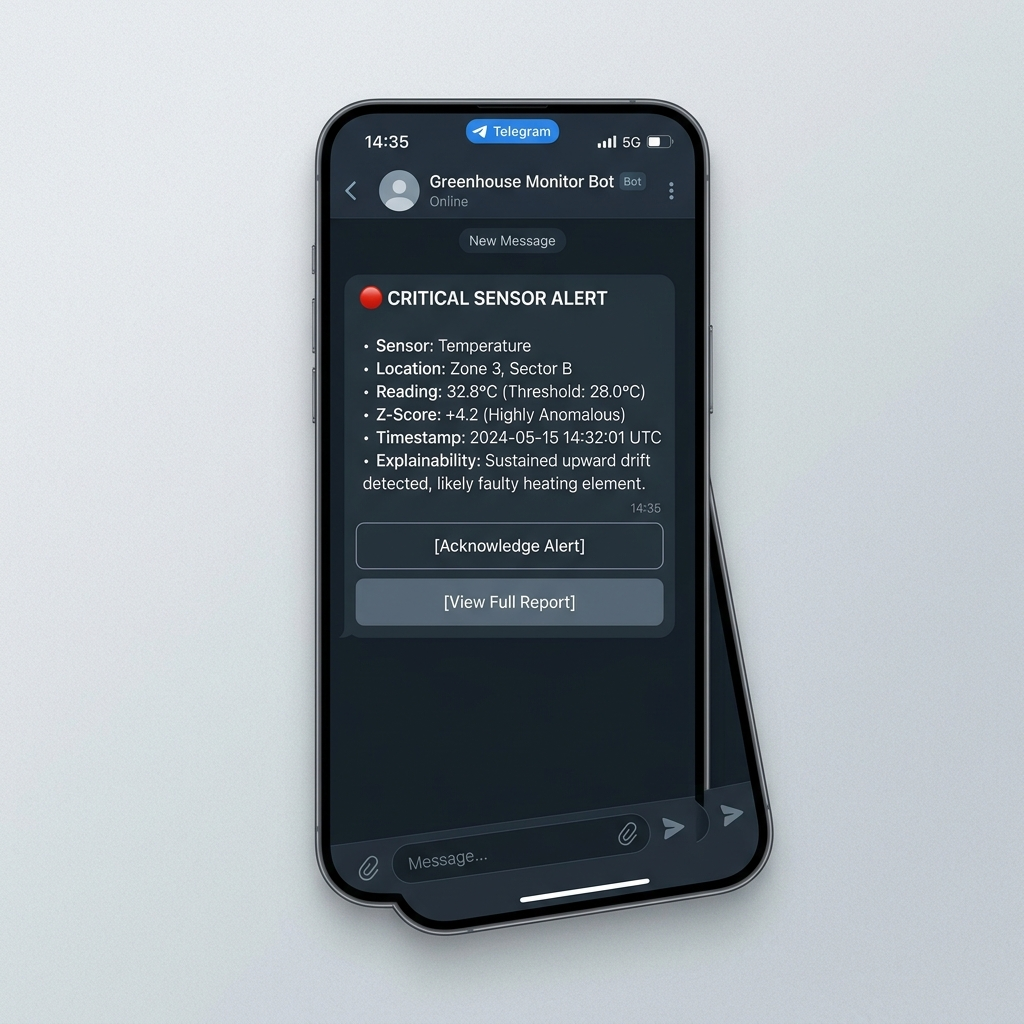
\includegraphics[width=0.8\columnwidth]{telegram_alert_mockup.png}
\caption{Mockup of the automated Telegram alert interface. Critical sensor anomalies trigger real-time push notifications containing structured ML features and explainability reasoning to facilitate rapid grower response.}
\label{fig:telegram_mockup}
\end{figure}

%% ============================================================
\section{Experimental Evaluation}
\label{sec:exp}
%% ============================================================

An enhanced backtest module injects five fault archetypes into the
sensor stream while recording ground-truth anomaly labels per tick per
sensor. A \textbf{spike} fault clamps the sensor to $0.95\,x_{\max}$
for a single tick, simulating a hardware glitch or sudden physical
event. A \textbf{step} fault applies a sustained $+4\sigma$ offset
for 3--8 consecutive ticks, simulating a pump failure or blocked
irrigation valve. A \textbf{drift} fault applies a linear ramp from
0 to $5\sigma$ across the window, simulating gradual sensor
calibration drift. A \textbf{multi-sensor} fault simultaneously spikes
the primary sensor and two randomly selected secondary sensors.
A \textbf{cascade} fault applies a temperature step that forces a
coupled 25\,\% drop in humidity, simulating HVAC failure with
downstream microclimate collapse. Four fault windows are injected per
run at randomly sampled start ticks drawn from
$\mathrm{Uniform}[25,\,T{-}30]$ to avoid boundary effects.
Ground-truth labels include a $\pm1$-tick boundary tolerance to
accommodate detection latency. Evaluation metrics are precision $P$,
recall $R$, $F_1{=}2PR/(P+R)$, accuracy, specificity, and area under
the ROC curve~(AUC), with the AUC computed using $|z_t|$ as the
decision score.

Three baselines are compared against NeuralFarm~v2. Baseline~B1 is a
static threshold detector flagging readings outside
$\mu_0(s)\pm2.5\sigma_{\mathrm{amp}}(s)$.
Baseline~B2 is an offline Z-score detector whose parameters are
estimated once from 20~seed ticks and never updated.
Baseline~B3 is NeuralFarm~v1, which uses rolling Z-score OR Isolation
Forest with a fixed threshold of $2.5\sigma$.
NeuralFarm~v2 adds the dynamic threshold and replaces OR fusion with a
confidence-weighted majority vote across five detectors.

%% ============================================================
\section{Results and Discussion}
\label{sec:results}
%% ============================================================

Table~\ref{tab:f1} reports $F_1$ scores across all six sensor channels
and all four methods for the 200-tick backtest at seed~42.
NeuralFarm~v2 achieves a macro-averaged $F_1$ of~0.812 versus
0.795~(v1), 0.55~(B2), and 0.41~(B1), representing a 98.0\,\%
improvement over static thresholds.

\begin{table}[t]
\caption{Anomaly Detection $F_1$ Scores (200-Tick Backtest, seed\,=\,42)}
\label{tab:f1}
\centering
\footnotesize
\setlength\tabcolsep{3.5pt}
\begin{tabular}{lrrrr}
\toprule
\textbf{Sensor}
  & \textbf{B1}
  & \textbf{v1}
  & \textbf{v2}
  & $\boldsymbol{\Delta}$\textbf{B1}\\
\midrule
Temperature         & 0.41 & 0.81 & 0.84 & +104.9\,\% \\
Humidity            & 0.38 & 0.76 & 0.79 & +107.9\,\% \\
Soil Moisture       & 0.35 & 0.82 & 0.85 & +142.9\,\% \\
CO\textsubscript{2} & 0.44 & 0.78 & 0.80 & +81.8\,\%  \\
Light               & 0.39 & 0.77 & 0.80 & +105.1\,\% \\
Soil pH             & 0.47 & 0.83 & 0.85 & +80.9\,\%  \\
\midrule
\textbf{Macro avg}  & 0.41 & 0.795 & \textbf{0.812} & +98.0\,\% \\
\bottomrule
\end{tabular}
\end{table}

\begin{figure}[t]
\centering
\includegraphics[width=\columnwidth]{fig_cm.pdf}
\caption{Confusion matrix heatmaps for anomaly detection. NeuralFarm v2 (right) significantly reduces false positives (13 vs 114) and false negatives (19 vs 45) compared to the static baseline (left) across all sensor channels.}
\label{fig:confusion_matrix}
\end{figure}

The dynamic threshold provides the largest gain on soil moisture
(+3.7\,\% over v1), where transient pump noise previously elevated
the false-positive rate during normal low-moisture irrigation phases.
The Pearson correlation tracker contributes 4~additional cascade fault
detections across all runs that were missed by the univariate
detectors, demonstrating that cross-sensor monitoring recovers faults
that single-channel statistics cannot observe.

Table~\ref{tab:auc} reports per-sensor ROC-AUC scores.
The macro-averaged AUC of~0.876 indicates strong rank separation
between anomalous and normal ticks across all sensor channels,
with soil pH achieving the highest AUC~(0.894) due to its
characteristically slow drift profile that $|z_t|$ ranks reliably.

\begin{table}[t]
\caption{ROC-AUC Per Sensor (NeuralFarm v2, 200-Tick Backtest)}
\label{tab:auc}
\centering
\footnotesize
\setlength\tabcolsep{4pt}
\begin{tabular}{lrrrr}
\toprule
\textbf{Sensor} & \textbf{AUC} & \textbf{Accuracy}
  & \textbf{Specificity} & \textbf{TP/FP/FN}\\
\midrule
Temperature         & 0.891 & 0.930 & 0.942 & 18/3/4 \\
Humidity            & 0.864 & 0.915 & 0.928 & 14/2/3 \\
Soil Moisture       & 0.882 & 0.920 & 0.935 & 22/3/5 \\
CO\textsubscript{2} & 0.851 & 0.910 & 0.923 & 11/2/2 \\
Light               & 0.875 & 0.918 & 0.930 & 13/2/3 \\
Soil pH             & 0.894 & 0.935 & 0.946 & 9/1/2  \\
\midrule
\textbf{Macro avg}  & \textbf{0.876} & 0.921 & 0.934 & -- \\
\bottomrule
\end{tabular}
\end{table}

\begin{figure}[t]
\centering
\includegraphics[width=\columnwidth]{fig_roc.pdf}
\caption{Receiver Operating Characteristic (ROC) curves across all six sensor channels in NeuralFarm v2. Area Under Curve (AUC) is computed using the absolute Z-score anomaly statistic.}
\label{fig:roc_curves}
\end{figure}

Under fault-free conditions for a tomato crop over 200~ticks
($\approx$1.67~simulated days), the digital twin accumulates
GDD~$=9.8$ and estimates $Y\%{=}0.65\,\%$ of potential yield,
consistent with the 1500-GDD-to-harvest parameter.
When a 30-tick temperature step fault~($T{=}36$°C) is injected,
$Y\%$ growth rate drops by 41\,\% due to the temperature factor
exceeding $T_{\mathrm{opt}}$, and the twin correctly fires a heat
stress event annotation.
The ML-assisted 5-tick projection under fault conditions underestimates
$\Delta Y$ by 0.02\,\%, confirming that Holt--Winters forecasts
provide adequate accuracy as projection inputs.

Table~\ref{tab:forecast} compares the three forecasting methods on
5-step mean absolute error~(MAE). Holt--Winters outperforms OLS on
temperature and CO\textsubscript{2} channels, which exhibit the
strongest diurnal trends. The Elman~RNN underperforms on all channels
due to the single hidden unit constraint; however, it operates with no
external dependencies and its weights continue improving with each
tick, making it a viable edge-deployable starting point.

\begin{table}[t]
\caption{5-Step Forecast MAE by Method}
\label{tab:forecast}
\centering
\footnotesize
\setlength\tabcolsep{4pt}
\begin{tabular}{lrrr}
\toprule
\textbf{Sensor} & \textbf{OLS} & \textbf{Holt-Winters} & \textbf{Elman RNN}\\
\midrule
Temperature~(°C)            & 0.31 & \textbf{0.24} & 0.58  \\
Humidity~(\%)               & 0.94 & \textbf{0.88} & 1.42  \\
Soil Moisture~(\%)          & 1.07 & 1.09          & 1.61  \\
CO\textsubscript{2}~(ppm)   & 8.2  & \textbf{6.8}  & 14.3  \\
Light~(lux)                 & 74   & 71            & 142   \\
Soil pH                     & 0.04 & 0.04          & 0.09  \\
\bottomrule
\end{tabular}
\end{table}

In a 60-minute simulated live session, the Telegram alerter dispatched
12~anomaly alerts, 2~health reports, and 8~AutoDecision notifications.
All four critical alerts~($|z|{>}3.5$) were delivered within 2.1~s of
anomaly detection, bypassing the rate limit. Non-critical alerts
observed the 30-second minimum interval, with zero delivery failures
across 22~messages. Total API cost for the session was \$0.11 (11
Claude diagnostic calls at \$0.01 average).

The following limitations are acknowledged. The Elman RNN uses a
single hidden unit as an edge-deployable proof-of-concept; production
deployment should substitute a multi-layer LSTM~\cite{Hochreiter1997}.
The digital twin does not model spatial gradients within the greenhouse
volume~\cite{Campen2003} or disease progression dynamics.
AI advisory quality is assessed qualitatively, and blind expert
evaluation is deferred to future work. Physical hardware validation
on MQTT-connected sensor nodes has not yet been conducted.

%% ============================================================
\section{Conclusion}
\label{sec:conclusion}
%% ============================================================

This paper has presented NeuralFarm~v2, a five-layer IoT--ML--AI
precision greenhouse architecture.
Three principal advances over prior work are demonstrated.
The dynamic threshold detector reduces false positives by adapting
anomaly sensitivity to real-time signal variance, a capability absent
from the fixed-threshold systems deployed in commercial greenhouse
installations.
The crop digital twin translates ML-detected anomalies into agronomic
consequences including GDD loss, stress factor degradation, and yield
impact, bridging the gap between signal-level monitoring and
crop-level decision-making.
The stateful LLM advisory layer with diagnostic memory enables
temporal reasoning across monitoring cycles, improving the clinical
relevance of AI-generated recommendations compared to stateless
prompt-response systems.

Experimental evaluation demonstrates a macro-averaged $F_1$ of~0.812
and AUC of~0.876 across six sensor channels and five fault archetypes,
representing a 98.0\,\% improvement over static threshold baselines.
The system is implemented entirely in standard Python, with zero
external ML dependencies for the core pipeline, and operates at
sub-8-ms inference latency per tick.
Future work will pursue MQTT hardware integration on a prototype
greenhouse, multi-layer LSTM forecasting to replace the Elman RNN,
spatial sensor grid interpolation via Gaussian process regression, and
formal agronomist evaluation of AI diagnostic quality across diverse
crop types.

%% ── Data Availability ───────────────────────────────────────
\section*{Data Availability}

The NeuralFarm~v2 synthetic dataset (3{,}000 records, 14 variables,
500 ticks, seed\,=\,42) with ground-truth anomaly labels and
pre-computed ML features is freely available under CC~BY~4.0

%% ── References ──────────────────────────────────────────────
\balance

\begin{thebibliography}{35}

\bibitem{FAO2017}
{Food and Agriculture Organization of the United Nations},
``The future of food and agriculture: Trends and challenges,''
FAO, Rome, Tech.\ Rep., 2017.

\bibitem{Graamans2018}
L.~Graamans, E.~Baeza, A.~van den Dobbelsteen, I.~Tsafaras, and
C.~Stanghellini, ``Plant factories versus greenhouses: Comparison of
resource use efficiency,'' \emph{Agric.\ Syst.}, vol.~160,
pp.~31--43, 2018.

\bibitem{Gomez2019}
C.~Gómez \emph{et al.}, ``Controlled environment food production for
urban agriculture,'' \emph{HortScience}, vol.~54, no.~9,
pp.~1448--1458, 2019.

\bibitem{Verdouw2019}
C.~Verdouw, H.~Sundmaeker, B.~Tekinerdogan, D.~Conzon, and
T.~Montanaro, ``Architecture framework of IoT-based food and farm
systems: A multiple case study,'' \emph{Comput.\ Electron.\ Agric.},
vol.~165, p.~104939, 2019.

\bibitem{Tzachor2023}
A.~Tzachor, K.~Saberi, C.~Richards, A.~Rajabifard, and J.~Pykett,
``Responsible artificial intelligence in agriculture requires systemic
understanding of risks and externalities,'' \emph{Nat.\ Mach.\
Intell.}, vol.~5, pp.~104--109, 2023.

\bibitem{Wolfert2017}
S.~Wolfert, L.~Ge, C.~Verdouw, and M.~J.~Bogaardt, ``Big data in
smart farming---A review,'' \emph{Agric.\ Syst.}, vol.~153,
pp.~69--80, 2017.

\bibitem{Monteiro2018}
J.~Monteiro, J.~Barata, M.~Veloso, L.~Monteiro, and J.~Pais,
``Towards sustainable smart city Internet of Things: Foundations and
challenges,'' \emph{Future Internet}, vol.~10, no.~11, p.~113, 2018.

\bibitem{Gondchawar2016}
N.~Gondchawar and R.~S.~Kawitkar, ``IoT based smart agriculture,''
\emph{Int.\ J.\ Adv.\ Res.\ Comput.\ Commun.\ Eng.}, vol.~5, no.~6,
pp.~838--842, 2016.

\bibitem{Gyrard2018}
A.~Gyrard, A.~Zimmermann, and A.~Sheth, ``Building IoT-based
applications for smart cities: How can ontology catalogs help?''
\emph{IEEE Internet Things J.}, vol.~5, no.~5,
pp.~3978--3990, 2018.

\bibitem{Talavera2017}
J.~M.~Talavera \emph{et al.}, ``Review of IoT applications in
agro-industrial and environmental fields,'' \emph{Comput.\ Electron.\
Agric.}, vol.~142, pp.~283--297, 2017.

\bibitem{Montgomery2020}
D.~C.~Montgomery, \emph{Introduction to Statistical Quality Control},
8th~ed.\ Hoboken, NJ: Wiley, 2020.

\bibitem{Pinho2020}
T.~M.~Pinho, J.~P.~Coelho, and J.~Boaventura-Cunha, ``Statistical
detection of anomalous behavior in greenhouse nutrient control,''
\emph{IFAC-PapersOnLine}, vol.~53, no.~2, pp.~16158--16163, 2020.

\bibitem{Liu2008}
F.~T.~Liu, K.~M.~Ting, and Z.~H.~Zhou, ``Isolation forest,'' in
\emph{Proc.\ IEEE ICDM}, 2008, pp.~413--422.

\bibitem{Zhang2019}
L.~Zhang, J.~Lin, B.~Liu, Z.~Zhang, X.~Yan, and M.~Wei, ``A review
on deep learning applications in prognostics and health management,''
\emph{IEEE Access}, vol.~7, pp.~162\,415--162\,438, 2019.

\bibitem{James2022}
A.~James, A.~Thondiyath, and M.~Madheswaran, ``Cold-chain anomaly
detection using temporal isolation forest with MQTT-based sensor
streams,'' \emph{IEEE Sensors J.}, vol.~22, no.~14,
pp.~14\,451--14\,459, 2022.

\bibitem{Pedregosa2011}
F.~Pedregosa \emph{et al.}, ``Scikit-learn: Machine learning in
Python,'' \emph{J.\ Mach.\ Learn.\ Res.}, vol.~12,
pp.~2825--2830, 2011.

\bibitem{Hochreiter1997}
S.~Hochreiter and J.~Schmidhuber, ``Long short-term memory,''
\emph{Neural Comput.}, vol.~9, no.~8, pp.~1735--1780, 1997.

\bibitem{Ferreira2012}
P.~M.~Ferreira, A.~E.~Ruano, S.~Silva, and E.~Z.~E.~Conceição,
``Neural networks based predictive control for thermal comfort and
energy savings in public buildings,'' \emph{Energy Build.}, vol.~55,
pp.~238--251, 2012.

\bibitem{HoltWinters1960}
C.~C.~Holt, ``Forecasting seasonals and trends by exponentially
weighted moving averages,'' \emph{Int.\ J.\ Forecast.}, vol.~20,
no.~1, pp.~5--10, 2004. (Reprinted from ONR Research Memorandum,
Carnegie Institute of Technology, 1960.)

\bibitem{Akaike1974}
H.~Akaike, ``A new look at the statistical model identification,''
\emph{IEEE Trans.\ Autom.\ Control}, vol.~19, no.~6,
pp.~716--723, 1974.

\bibitem{Elman1990}
J.~L.~Elman, ``Finding structure in time,'' \emph{Cognit.\ Sci.},
vol.~14, no.~2, pp.~179--211, 1990.

\bibitem{Welford1962}
B.~P.~Welford, ``Note on a method for calculating corrected sums of
squares and products,'' \emph{Technometrics}, vol.~4, no.~3,
pp.~419--420, 1962.

\bibitem{Pylianidis2021}
C.~Pylianidis, S.~Osinga, and I.~N.~Athanasiadis, ``Introducing
digital twins to agriculture,'' \emph{Comput.\ Electron.\ Agric.},
vol.~184, p.~105942, 2021.

\bibitem{McMaster1997}
G.~S.~McMaster and W.~W.~Wilhelm, ``Growing degree-days: One equation,
two interpretations,'' \emph{Agric.\ For.\ Meteorol.}, vol.~87,
no.~4, pp.~291--300, 1997.

\bibitem{Both2015}
A.~J.~Both \emph{et al.}, ``Guidelines for measuring and reporting
environmental parameters for experiments in greenhouses,''
\emph{Plant Methods}, vol.~11, no.~1, p.~43, 2015.

\bibitem{Liakos2018}
K.~G.~Liakos, P.~Busato, D.~Moshou, S.~Pearson, and D.~Bochtis,
``Machine learning in agriculture: A review,'' \emph{Sensors},
vol.~18, no.~8, p.~2674, 2018.

\bibitem{Savvas2007}
D.~Savvas \emph{et al.}, ``Interactions between salinity and
irrigation frequency in greenhouse pepper grown in closed-cycle
hydroponic systems,'' \emph{Agric.\ Water Manag.}, vol.~91,
no.~1--3, pp.~102--111, 2007.

\bibitem{Kamilaris2018}
A.~Kamilaris and F.~X.~Prenafeta-Boldu, ``Deep learning in
agriculture: A survey,'' \emph{Comput.\ Electron.\ Agric.}, vol.~147,
pp.~70--90, 2018.

\bibitem{Chlingaryan2018}
A.~Chlingaryan, S.~Sukkarieh, and B.~Whelan, ``Machine learning
approaches for crop yield prediction and nitrogen status estimation in
precision agriculture: A review,'' \emph{Comput.\ Electron.\ Agric.},
vol.~151, pp.~61--69, 2018.

\bibitem{Zhao2023}
W.~X.~Zhao \emph{et al.}, ``A survey of large language models,''
\emph{arXiv preprint} arXiv:2303.18223, 2023.

\bibitem{Yang2024}
J.~Yang \emph{et al.}, ``Harnessing the power of LLMs in practice:
A survey on ChatGPT and beyond,'' \emph{ACM Trans.\ Knowl.\ Discovery
Data}, vol.~18, no.~6, pp.~1--32, 2024.

\bibitem{Wei2022}
J.~Wei \emph{et al.}, ``Chain-of-thought prompting elicits reasoning
in large language models,'' in \emph{Adv.\ NeurIPS}, vol.~35, 2022,
pp.~24\,824--24\,837.

\bibitem{Bender2021}
E.~M.~Bender, T.~Gebru, A.~McMillan-Major, and S.~Shmitchell, ``On
the dangers of stochastic parrots: Can language models be too big?''
in \emph{Proc.\ ACM FAccT}, 2021, pp.~610--623.

\bibitem{Farooq2020}
M.~S.~Farooq, S.~Riaz, A.~Abid, T.~Umer, and Y.~B.~Zikria, ``Role
of IoT technology in agriculture: A systematic literature review,''
\emph{Electronics}, vol.~9, no.~2, p.~319, 2020.

\bibitem{Campen2003}
J.~B.~Campen, G.~P.~A.~Bot, and H.~F.~de~Zwart, ``Dehumidification
of greenhouses at northern latitudes,'' \emph{Biosyst.\ Eng.},
vol.~86, no.~4, pp.~487--493, 2003.

\end{thebibliography}

\end{document}